\documentclass[runningheads]{llncs}
\usepackage[T1]{fontenc}
\usepackage{graphicx}
\usepackage{booktabs}
\usepackage{multirow}
\usepackage{amsmath}
\usepackage{url}
\usepackage[hidelinks]{hyperref}
\graphicspath{{figures/}}
\pagestyle{plain}
\raggedbottom
\setlength{\textfloatsep}{5pt plus 1pt minus 2pt}
\setlength{\floatsep}{5pt plus 1pt minus 2pt}
\setlength{\intextsep}{5pt plus 1pt minus 2pt}
\setlength{\abovecaptionskip}{4pt}
\setlength{\belowcaptionskip}{1pt}
\renewcommand{\topfraction}{0.92}
\renewcommand{\bottomfraction}{0.80}
\renewcommand{\textfraction}{0.06}
\renewcommand{\floatpagefraction}{0.82}
\setcounter{topnumber}{3}
\setcounter{bottomnumber}{2}
\setcounter{totalnumber}{4}
\begin{document}

\title{PlasmaXAI: Counterfactual-Guided Explainable Fusion for Plasma Cell Recognition in Multiple Myeloma}
\titlerunning{PlasmaXAI}
\author{Arnob Aich Anurag}
\institute{American International University-Bangladesh, Dhaka, Bangladesh}
\authorrunning{Anurag et al.}

\maketitle
\thispagestyle{plain}

\begin{abstract}
Recognizing malignant plasma cells is important for multiple myeloma screening, yet manual microscopic review remains slow. This paper presents PlasmaXAI, an explainable digital pathology framework that combines frozen ResNet50 and DenseNet121 embeddings with handcrafted morphology, a morphology-derived counterfactual boundary model, and learned fusion gates that inject counterfactual information directly into the final decision pathway. Evaluated on PCMMD, PlasmaXAI achieved 93.42\% accuracy, 93.43\% weighted F1, 91.24\% plasma precision, 94.63\% plasma recall, and 97.76\% AUC at the selected operating point. The framework also produced counterfactual, calibration, ablation, and exploratory patient-level analyses. These findings position PlasmaXAI as an interpretable screening framework for digital hematopathology.
\keywords{Multiple myeloma \and Digital pathology \and Explainable AI \and Counterfactual analysis \and Plasma cell recognition \and Deep learning}
\end{abstract}

\section{Introduction}
Multiple myeloma is a hematologic malignancy characterized by abnormal plasma-cell proliferation in bone marrow, and morphologic assessment remains central to diagnosis, disease monitoring, and treatment planning \cite{mmreview}. In many laboratories, stained marrow smears are still reviewed manually. This workflow is labor-intensive, sensitive to stain variation, and vulnerable to reader-to-reader disagreement.

Recent progress in computational pathology suggests that deep learning can reduce this burden, but strong accuracy alone is not sufficient for clinical use \cite{litjens,bera,campanella}. A clinically useful plasma-cell system should support review rather than replace it; therefore, it must expose why it predicts malignancy and which features would change the decision.

PlasmaXAI was developed with that requirement in mind. Instead of attaching explanations after prediction, the framework integrates counterfactual morphology information into a learned fusion network so that explainability contributes directly to classification. The study makes three main contributions. First, it introduces an explainable multi-branch architecture for malignant plasma-cell recognition that combines deep image embeddings and interpretable morphology. Second, it embeds counterfactual distance and feature-shift signals inside the fusion pathway rather than treating them as post-hoc artifacts. Third, it evaluates the system beyond conventional accuracy using ablation, calibration, bootstrap confidence intervals, and exploratory patient-level robustness analysis.

\section{Literature Review}
Deep learning has become the dominant approach in digital pathology because convolutional models can capture cell texture, chromatic variation, and structural context more effectively than handcrafted descriptors alone \cite{litjens,janowczyk}. Studies in computational oncology show that clinically useful pathology systems must balance fine local detail with robust higher-level semantics across varying staining conditions \cite{bera,campanella}. Residual networks support deeper optimization through identity mappings, while densely connected networks improve feature reuse and gradient propagation \cite{resnet,densenet}. These backbone families are therefore well suited to plasma-cell images, where subtle nuclear irregularity, chromatin behavior, and cytoplasmic staining all contribute to malignancy recognition.

Explainability research in medical AI has progressed through local surrogates, saliency maps, attribution methods, and counterfactual reasoning \cite{lime,gradcam,shap,wachter}. Counterfactual explanations are particularly attractive in healthcare because they answer a clinically intuitive question: what minimal change would move a prediction toward a different class? DICE extends this idea by generating diverse counterfactual sets that improve interpretive coverage \cite{diceml}. Calibration is another important requirement, because a probability score has clinical value only when confidence aligns with observed frequency \cite{calibration}. Few systems make counterfactual information part of the decision path itself. PlasmaXAI addresses that gap by combining deep image features, interpretable morphology, and counterfactual-guided learned fusion in one screening framework.

\section{Materials and Methods}
\subsection{Dataset, Preprocessing, and Morphology Features}
Experiments were conducted on PCMMD using a cell-level classification set and a separate patient-organized cohort for exploratory patient analysis. Cell images were resized to 224 $\times$ 224 for CNN feature extraction. In parallel, a handcrafted morphology pipeline computed nucleus-to-cytoplasm ratio, nucleus area, cytoplasm area, roundness, staining intensity, granularity, and mean RGB channels. These descriptors form an interpretable phenotype layer that complements the learned image embeddings and supports counterfactual analysis.

\subsection{PlasmaXAI Architecture}
PlasmaXAI uses frozen ResNet50 and DenseNet121 encoders as complementary image branches. A logistic morphology model estimates a decision boundary in handcrafted feature space, from which the framework derives counterfactual distance and feature-shift terms that summarize how far a sample lies from the benign region and which morphology changes would most strongly alter the decision.

These signals are passed to a learned fusion module that separately encodes ResNet, DenseNet, morphology, counterfactual, and score streams. Counterfactual features modulate the image branches through sigmoid gates and also contribute to a softmax-based modality gate that controls the final weighted fusion. This design makes counterfactual reasoning structurally relevant to prediction rather than merely descriptive after prediction. Figure~\ref{fig:workflow} presents the overall workflow and Figure~\ref{fig:archdetail} shows the internal architecture in larger detail.

\begin{figure}[t]
\centering
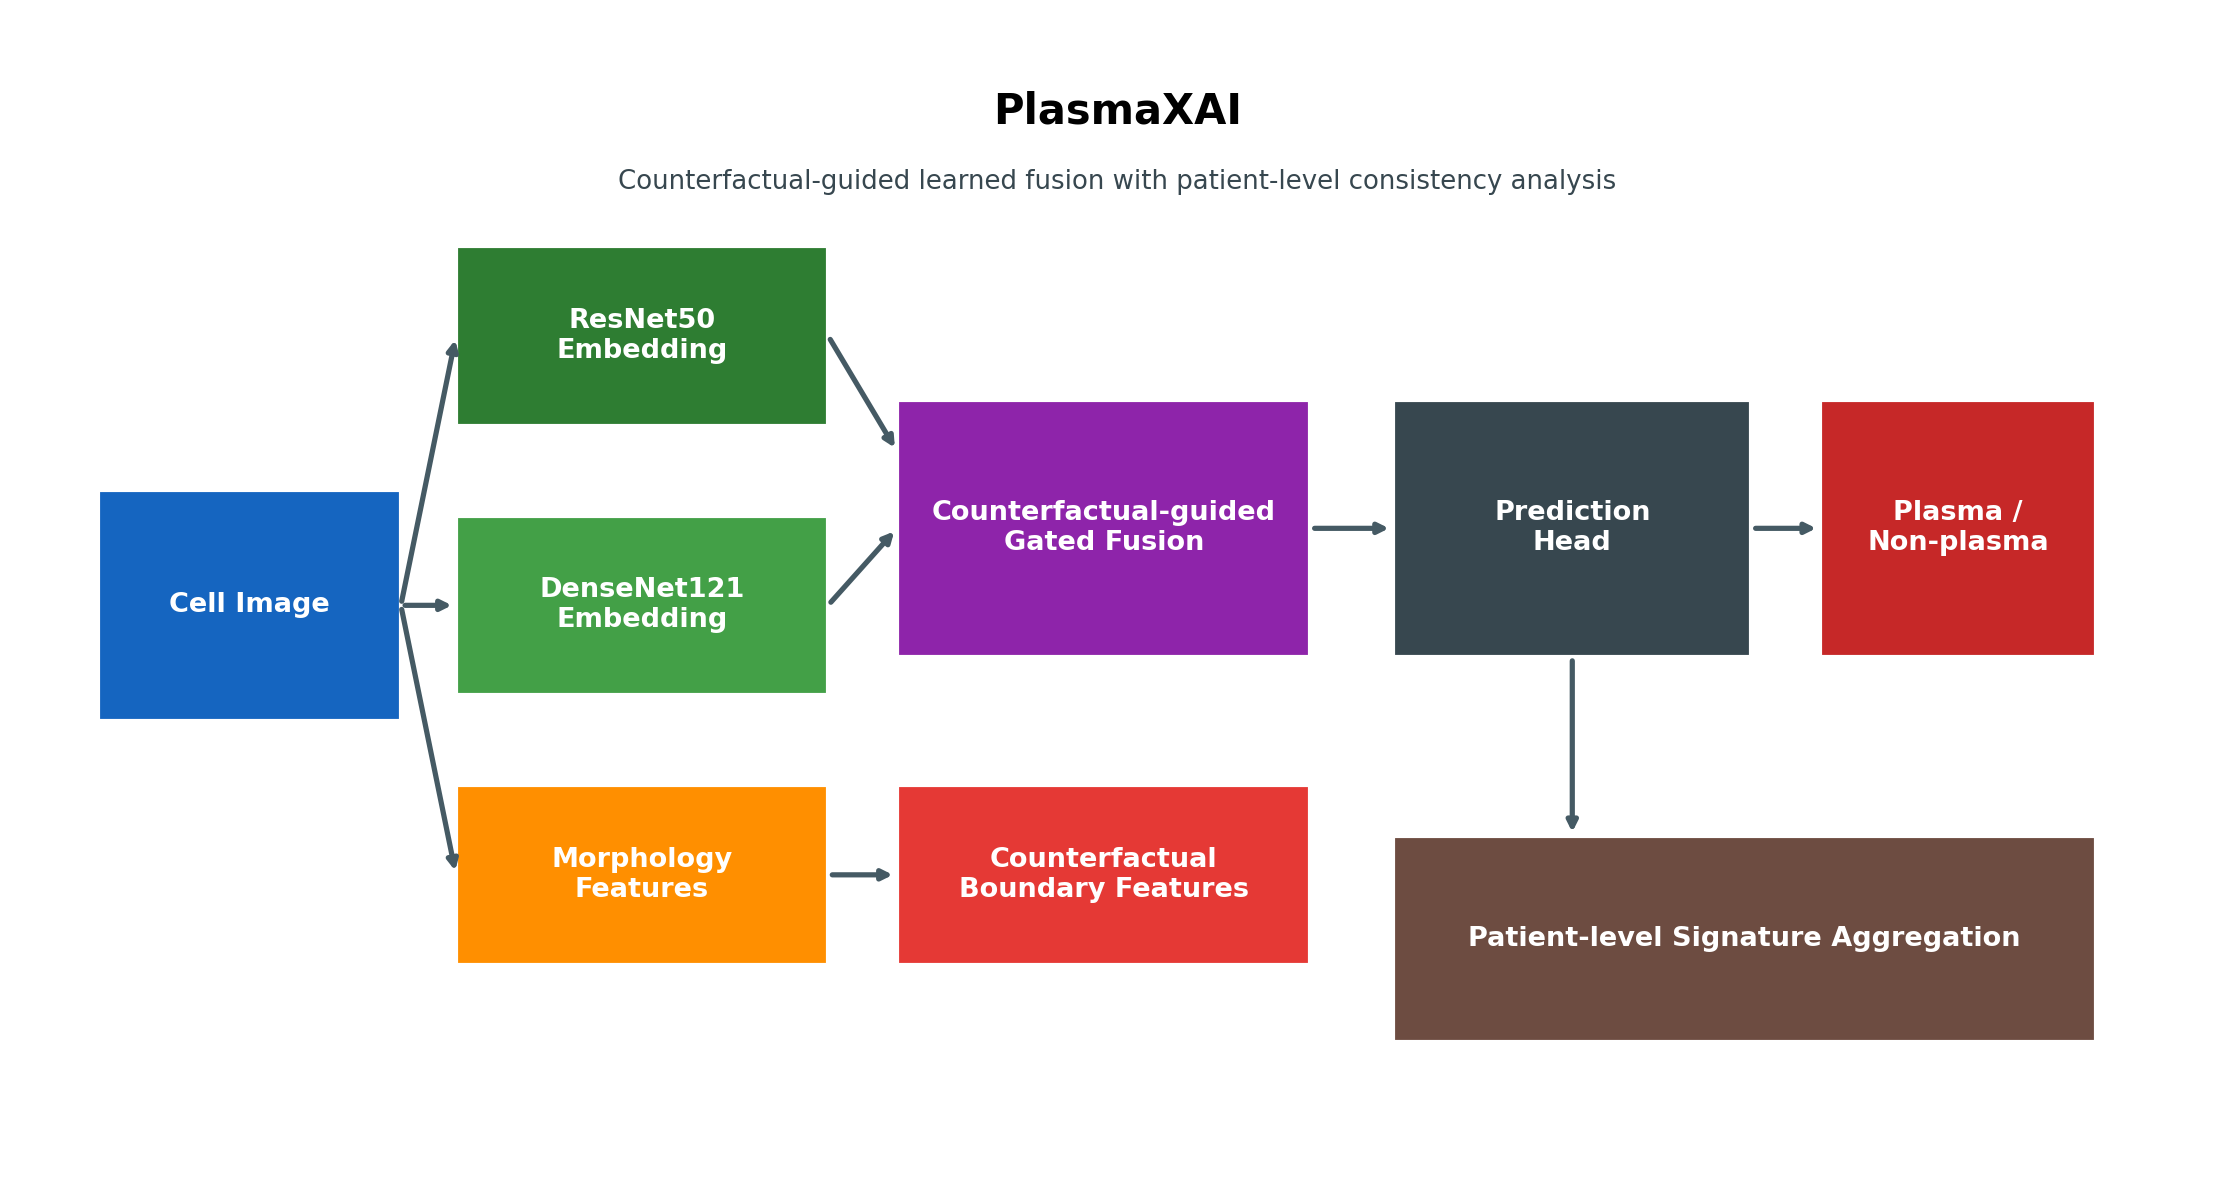
\includegraphics[width=0.93\textwidth,height=0.28\textheight,keepaspectratio]{plasmaxai_framework.png}
\caption{End-to-end PlasmaXAI workflow from image preprocessing to explainable prediction.}
\label{fig:workflow}
\end{figure}
Figure~\ref{fig:workflow} outlines the full processing pipeline used to generate predictions, explanations, and patient-level outputs.

\begin{figure}[t]
\centering
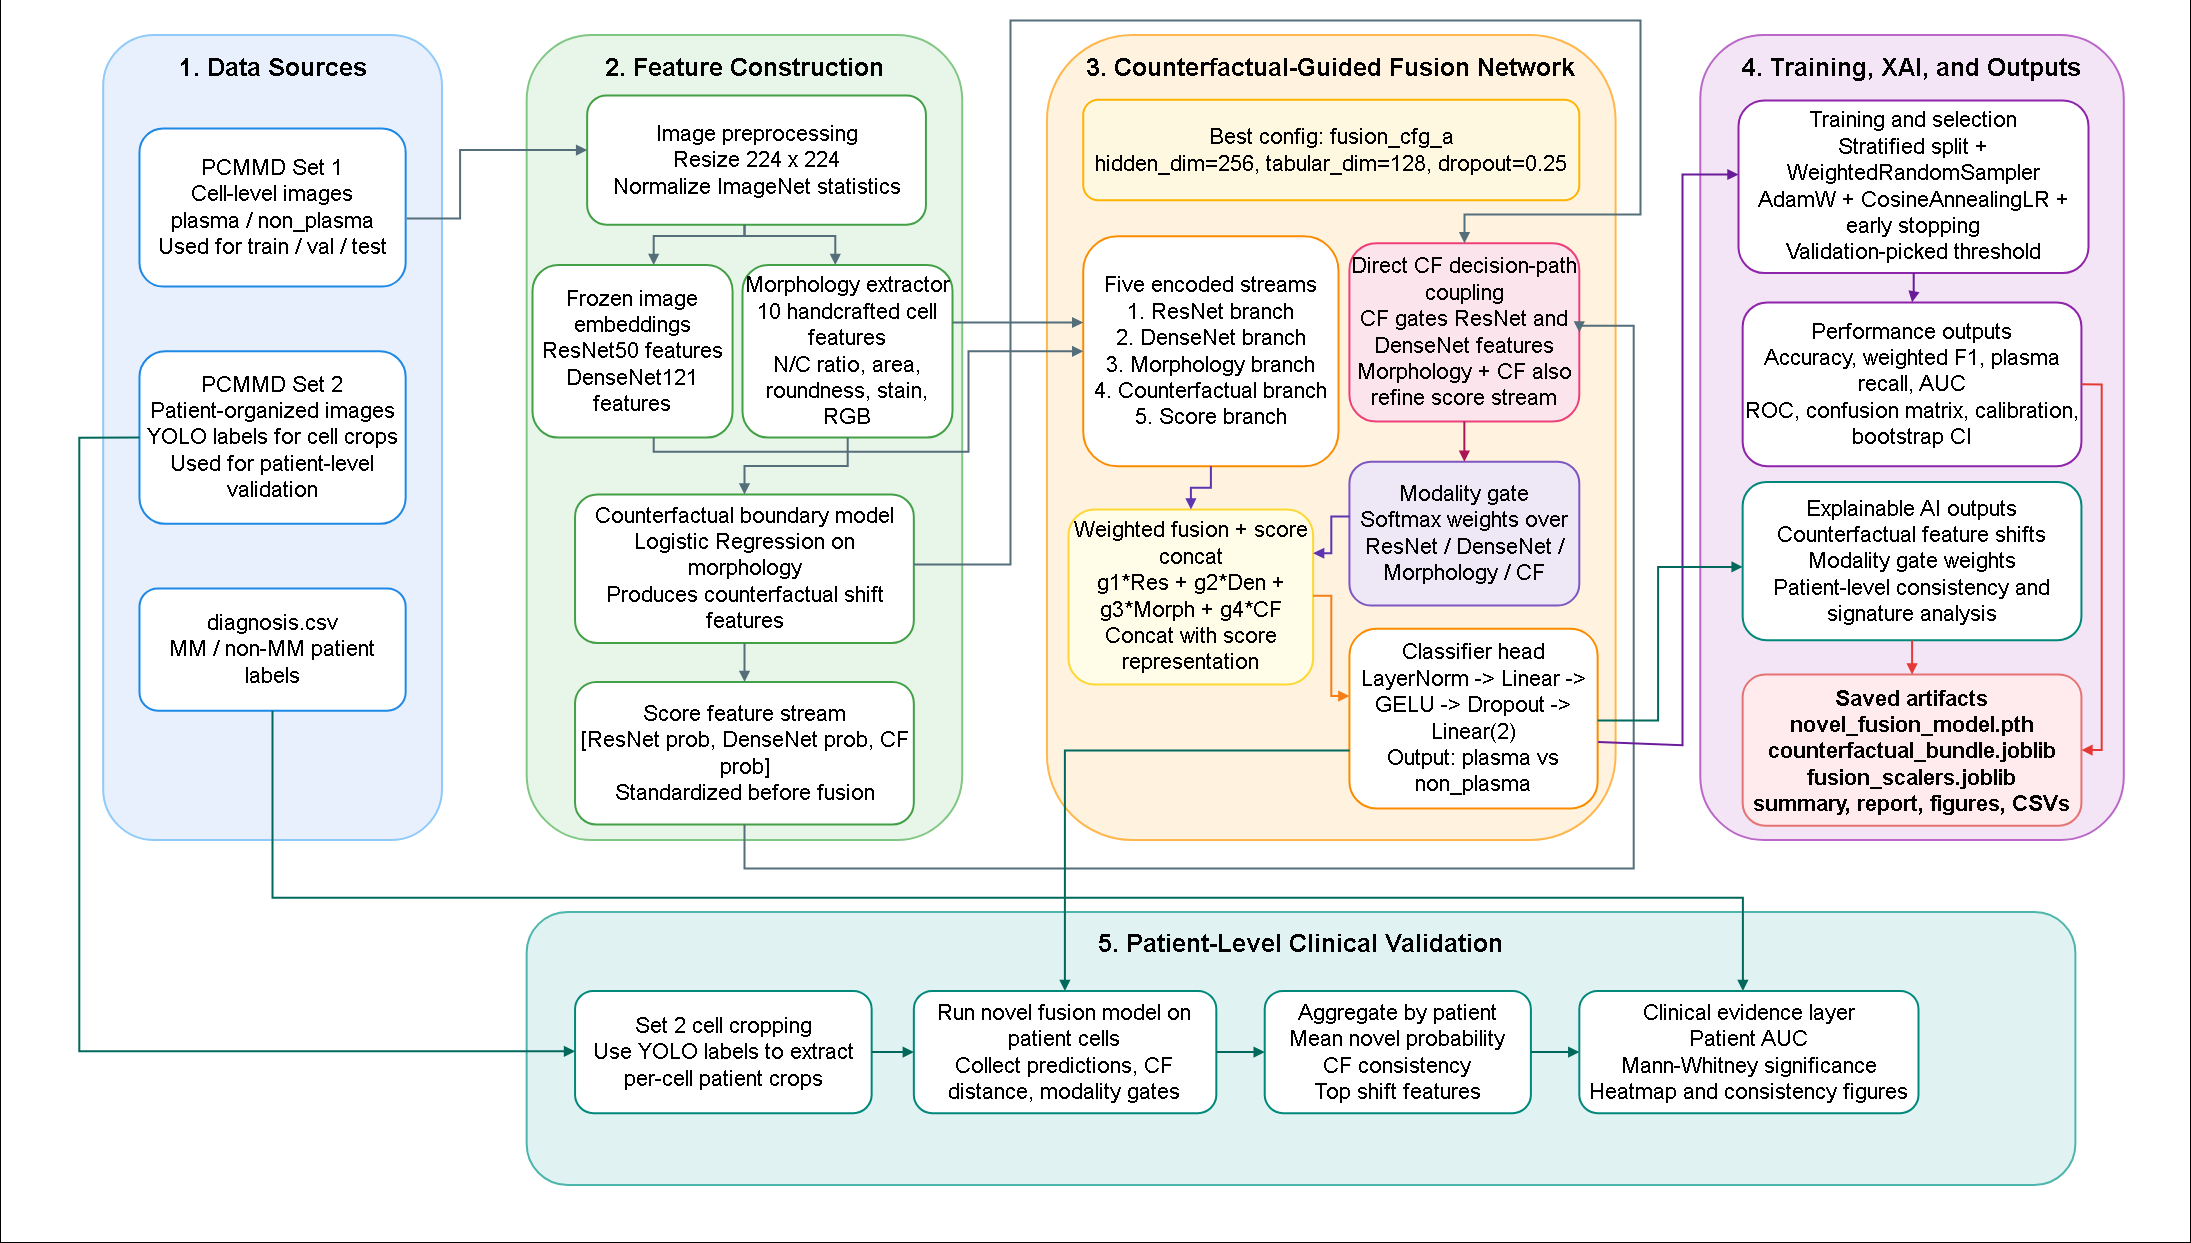
\includegraphics[width=0.93\textwidth,height=0.30\textheight,keepaspectratio]{Architecture_diagram.png}
\caption{Detailed internal PlasmaXAI fusion architecture with image, morphology, and counterfactual branches.}
\label{fig:archdetail}
\end{figure}
Figure~\ref{fig:archdetail} emphasizes that counterfactual features are inserted into the fusion process itself rather than appended only after classification.

\subsection{Training and Evaluation}
The deployment operating point was selected on validation data using a precision-recall balanced criterion. Final evaluation reports accuracy, weighted F1, plasma precision, plasma recall, and AUC. The study also includes ablation, bootstrap confidence intervals, calibration curves, exact patient-level permutation testing, and leave-one-patient-out robustness checks.

\section{Results and Discussion}
\subsection{Benchmark Performance}
At the selected operating point, PlasmaXAI achieved 93.42\% accuracy, 93.43\% weighted F1, 91.24\% plasma precision, 94.63\% plasma recall, and 97.76\% AUC. It therefore surpassed the strongest non-PlasmaXAI baselines on the three most deployment-relevant classification criteria: accuracy, precision, and recall. ResNet50 remained the strongest single deep backbone, while the previous optimized hybrid remained the strongest non-PlasmaXAI precision baseline.

\begin{table}[t]
\centering
\caption{Held-out test performance for the strongest comparison models.}
\label{tab:mainresults}
\small
\begin{tabular}{lccccc}
\toprule
Model & Acc. & F1 & Prec. & Rec. & AUC \\
\midrule
ResNet50 & 91.92 & 91.93 & 89.02 & 93.80 & 97.05 \\
Prev Hybrid & 91.73 & 91.73 & 90.91 & 90.91 & 97.12 \\
DenseNet121 & 89.85 & 89.83 & 90.17 & 87.19 & 96.36 \\
\textbf{PlasmaXAI} & \textbf{93.42} & \textbf{93.43} & \textbf{91.24} & \textbf{94.63} & \textbf{97.76} \\
\bottomrule
\end{tabular}
\end{table}

\begin{figure}[t]
\centering
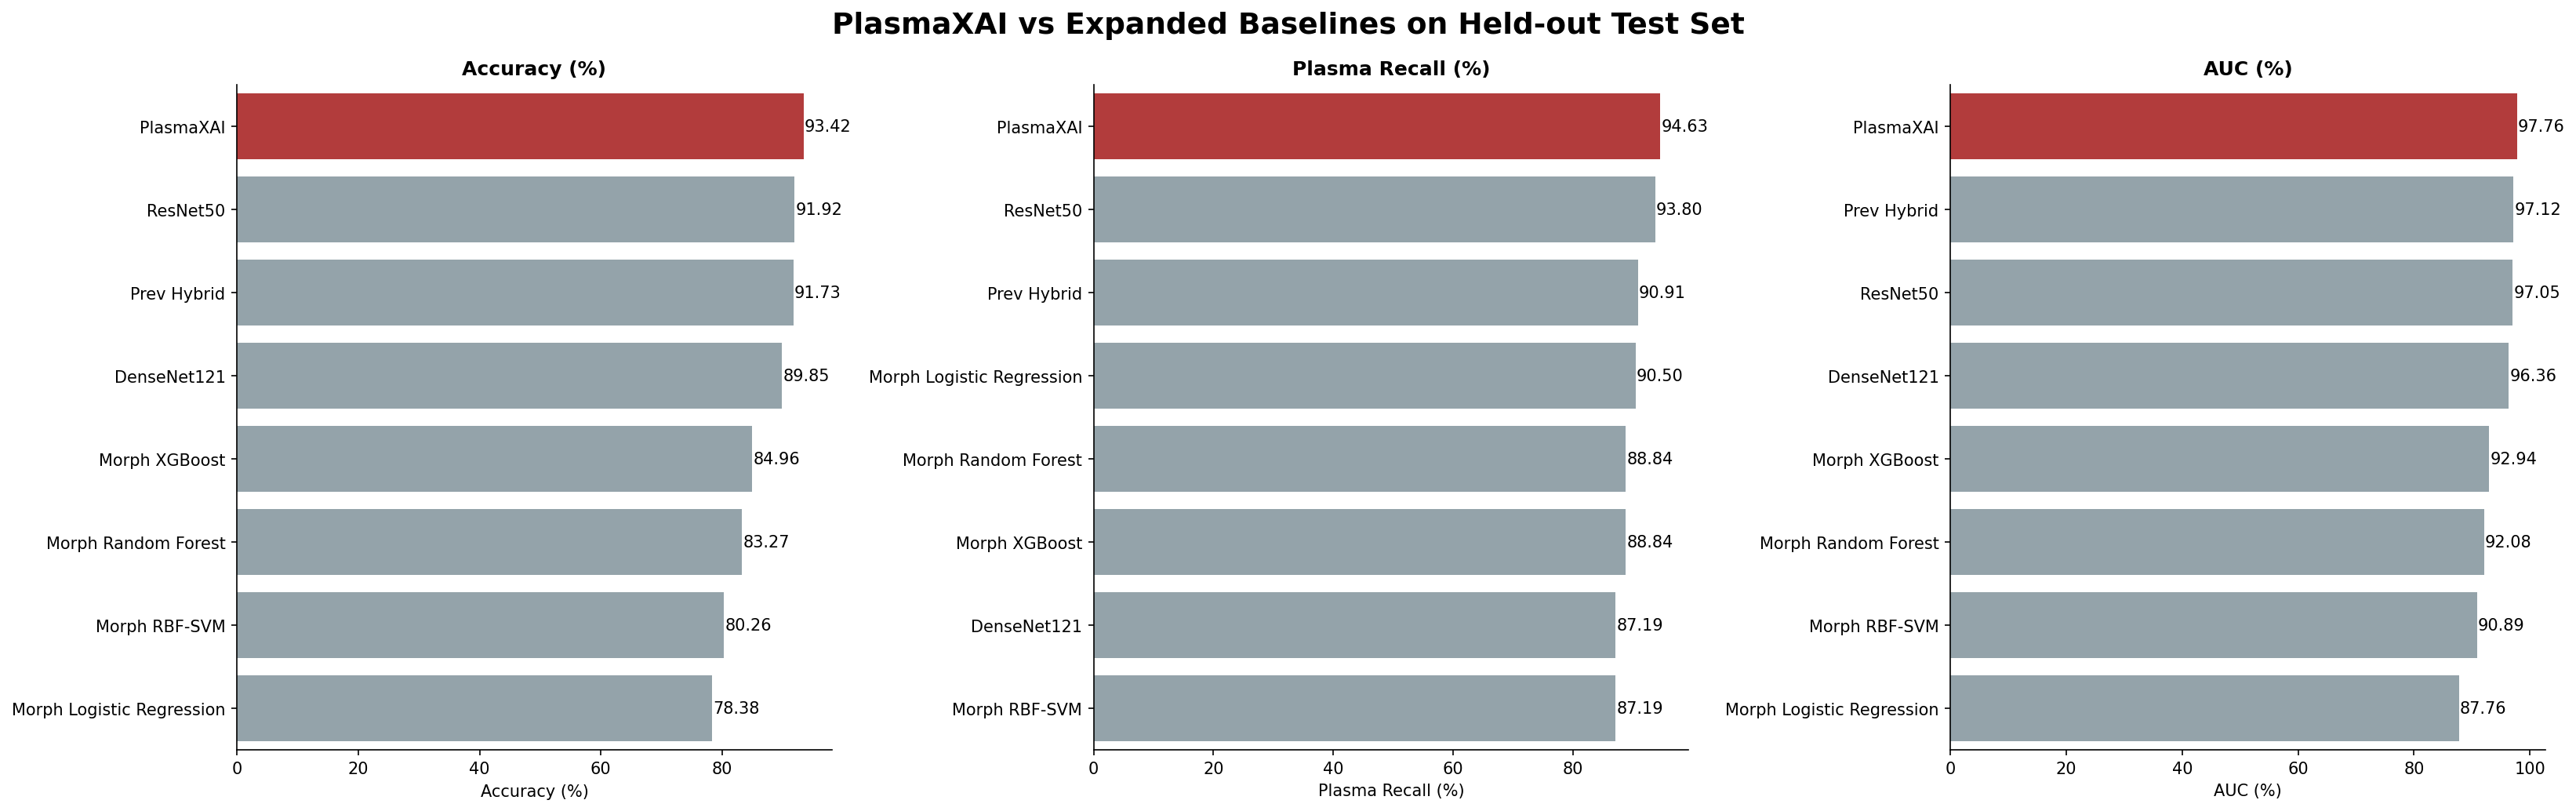
\includegraphics[width=0.93\textwidth,height=0.27\textheight,keepaspectratio]{plasmaxai_model_comparison.png}
\caption{Expanded benchmark comparison showing PlasmaXAI against deep and morphology-based baselines.}
\label{fig:modelcomp}
\end{figure}
Figure~\ref{fig:modelcomp} shows that the full framework delivers the strongest balance across the main benchmark metrics rather than improving one measure at the expense of another.

Bootstrap analysis indicated that the selected operating point was stable, with a 95\% confidence interval of 91.16--95.30 for accuracy, 91.30--97.20 for plasma recall, and 96.56--98.63 for AUC. This matters because a reliable screening aid should not depend on one favorable split.

\subsection{Explainability and Ablation}
The explainability pathway is a defining characteristic of PlasmaXAI. Counterfactual analysis identifies the morphology shifts most responsible for malignant predictions while also showing how the learned gates redistribute attention across image and tabular streams. In practical terms, the system produces both a malignant probability and an explanation of which feature changes would move the case toward a benign boundary.

\begin{figure}[t]
\centering
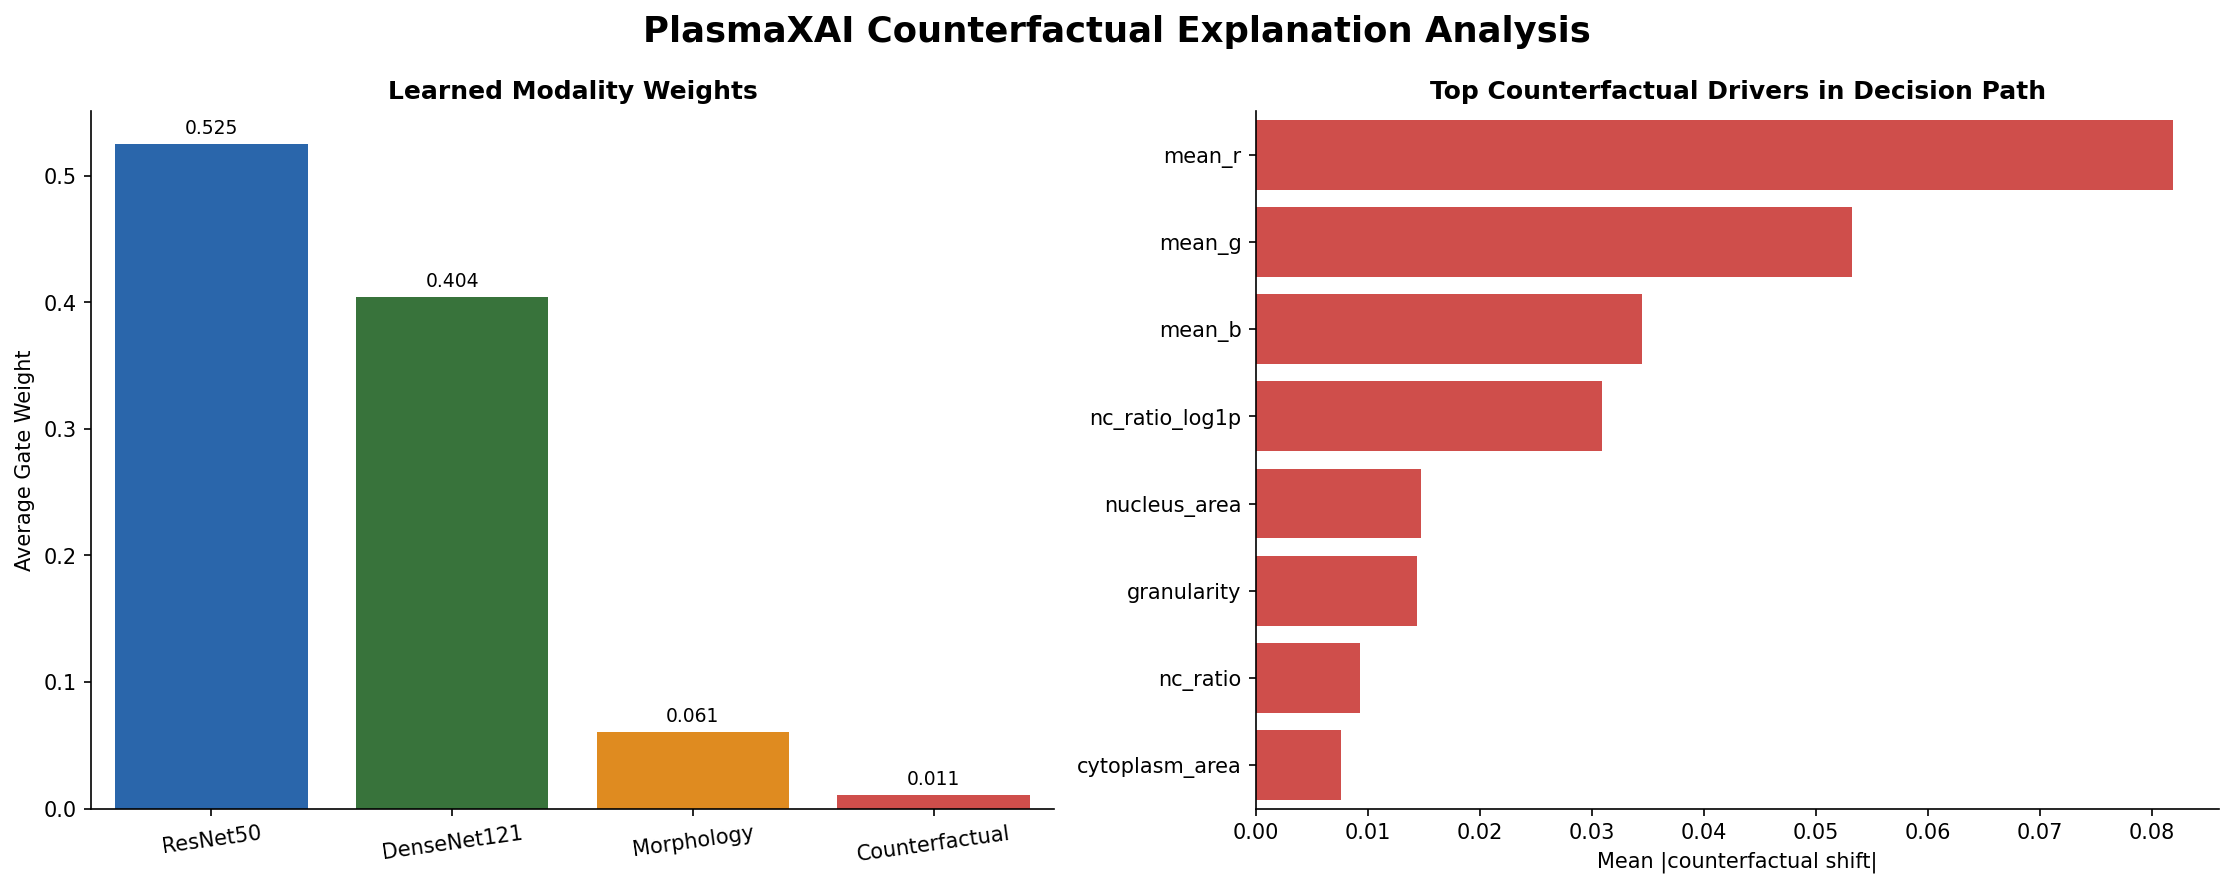
\includegraphics[width=0.90\textwidth,height=0.25\textheight,keepaspectratio]{plasmaxai_counterfactual.png}
\caption{Counterfactual explanation analysis for PlasmaXAI.}
\label{fig:counterfactual}
\end{figure}
Figure~\ref{fig:counterfactual} shows the feature-shift directions and modality-gating behavior that support a malignant decision.

\begin{figure}[t]
\centering
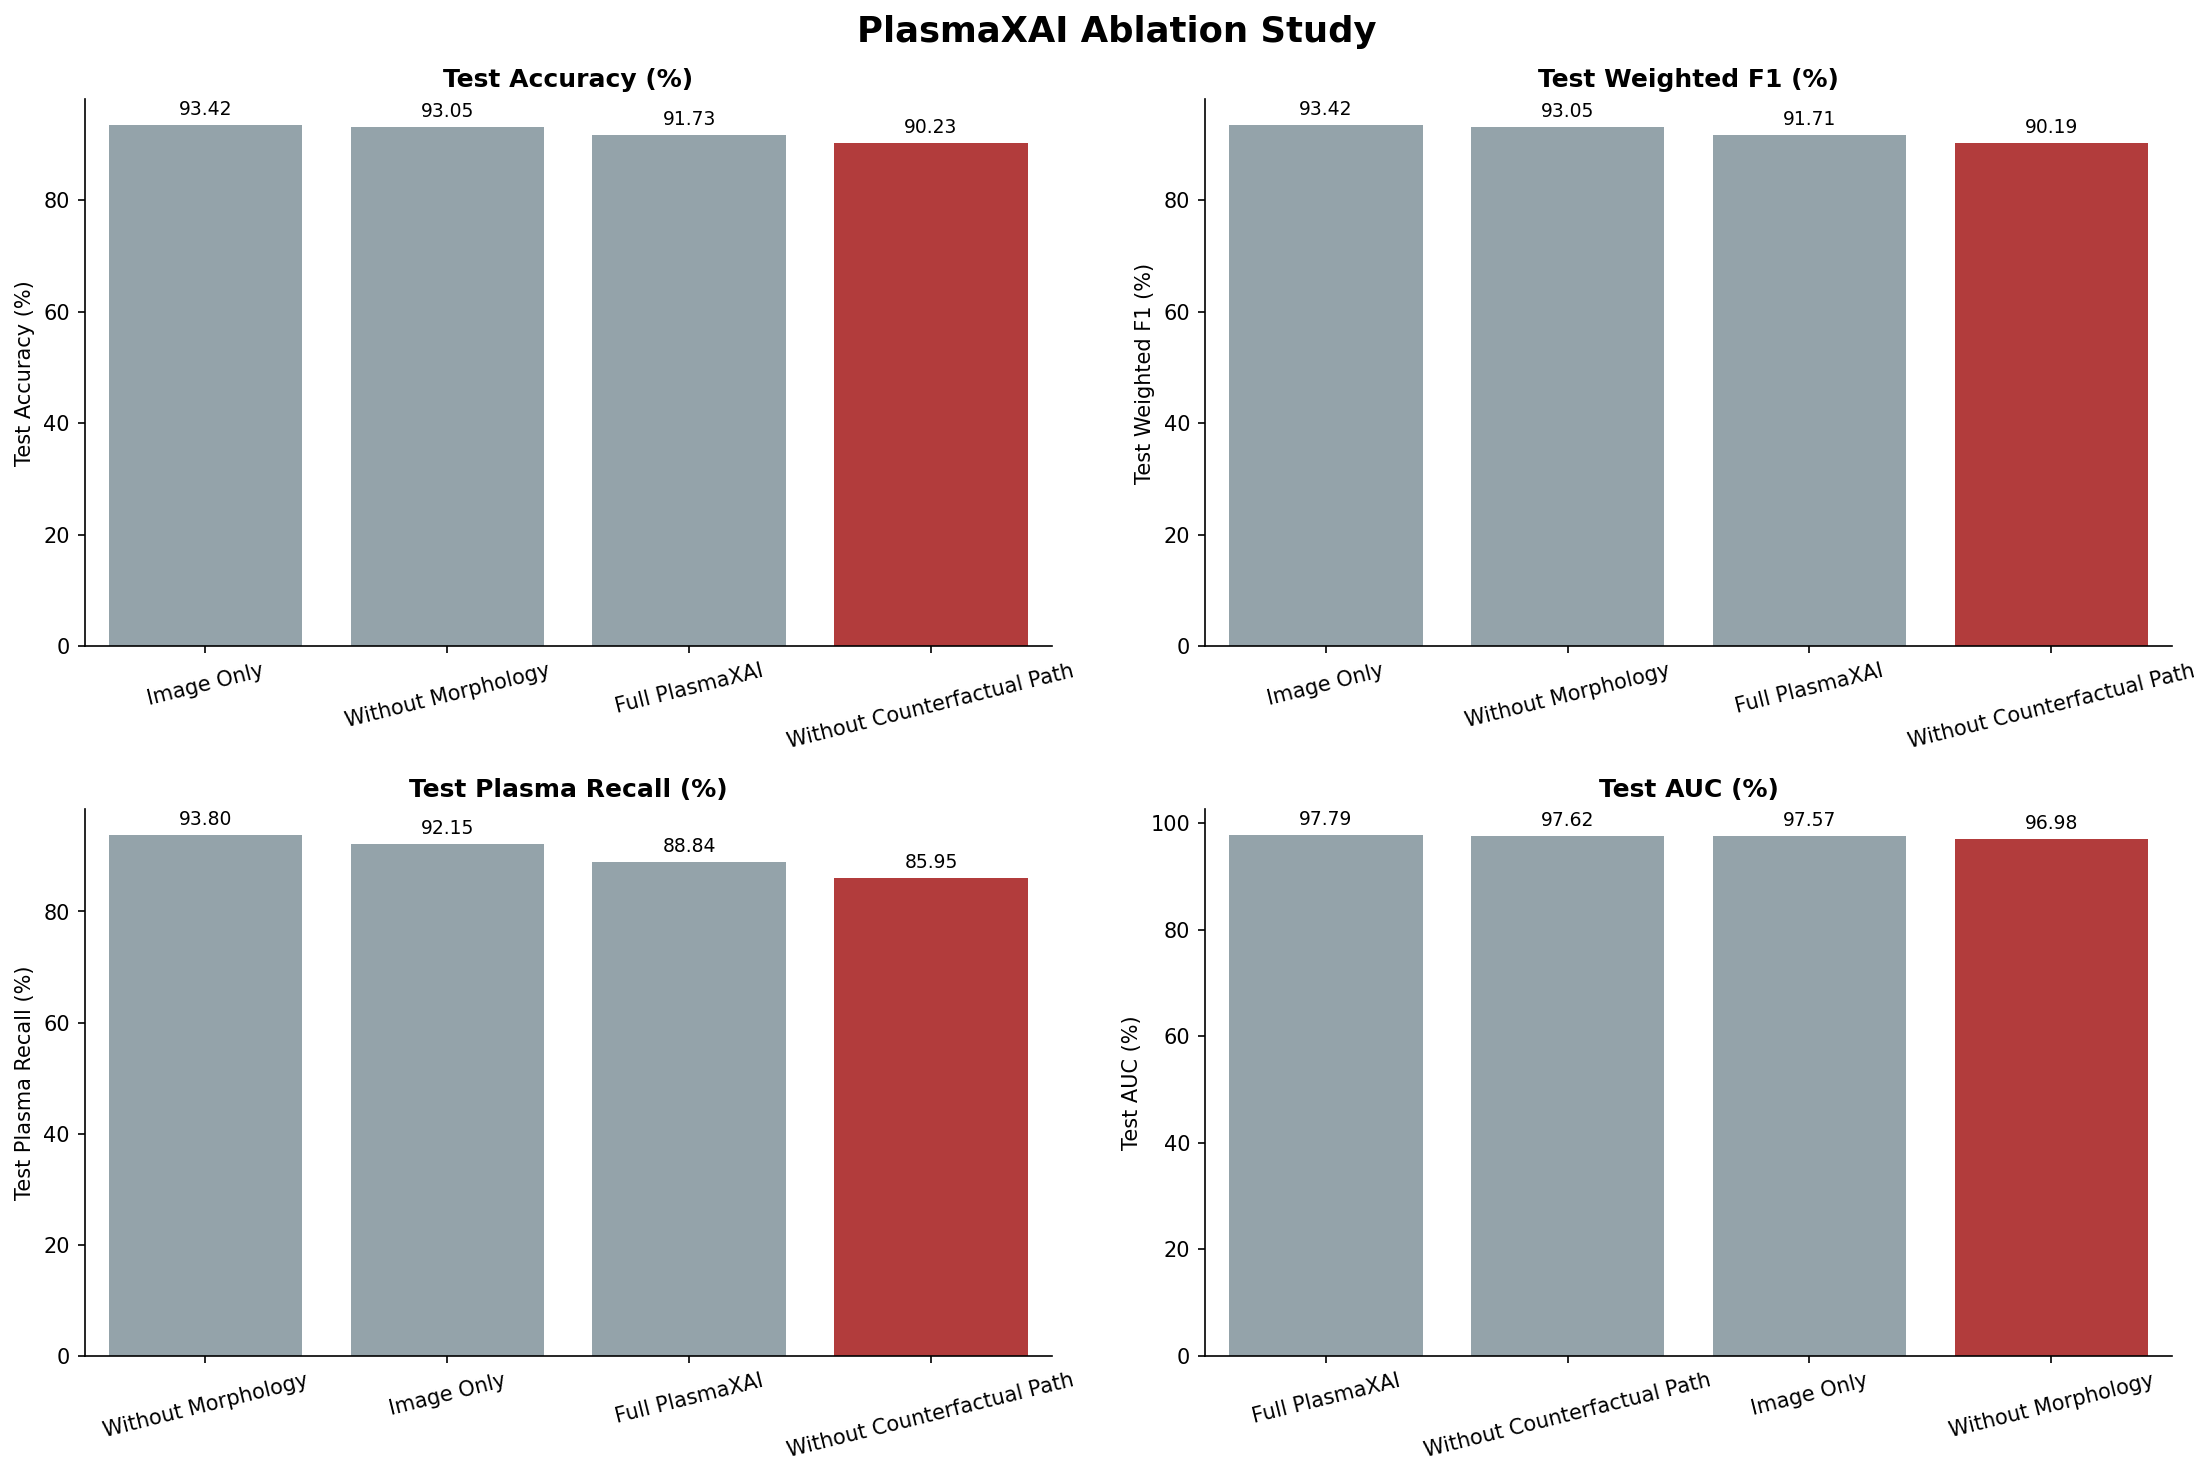
\includegraphics[width=0.90\textwidth,height=0.25\textheight,keepaspectratio]{plasmaxai_ablation.png}
\caption{Ablation study showing the effect of removing key PlasmaXAI components.}
\label{fig:ablation}
\end{figure}
Figure~\ref{fig:ablation} shows that removing the counterfactual branch causes the largest drop in malignant-cell recall.

The ablation results support this interpretation. Removing the counterfactual path reduced malignant recall to 85.95\%, far below the full model, while removing morphology also degraded performance. These results suggest that the primary gain comes from structured interaction between deep image features and counterfactual morphology reasoning, not from any single CNN backbone alone.

\subsection{Reliability and Patient-Level Signals}
Internal reliability analysis remained favorable. Exact permutation testing on the exploratory patient cohort produced p-values of 0.0040 (one-sided) and 0.0079 (two-sided), while the leave-one-patient-out patient AUC remained 1.000. Even so, this result should be interpreted carefully because the cohort is small and internally sourced. The patient-level analysis is therefore presented as encouraging, not definitive clinical validation.

\begin{figure}[t]
\centering
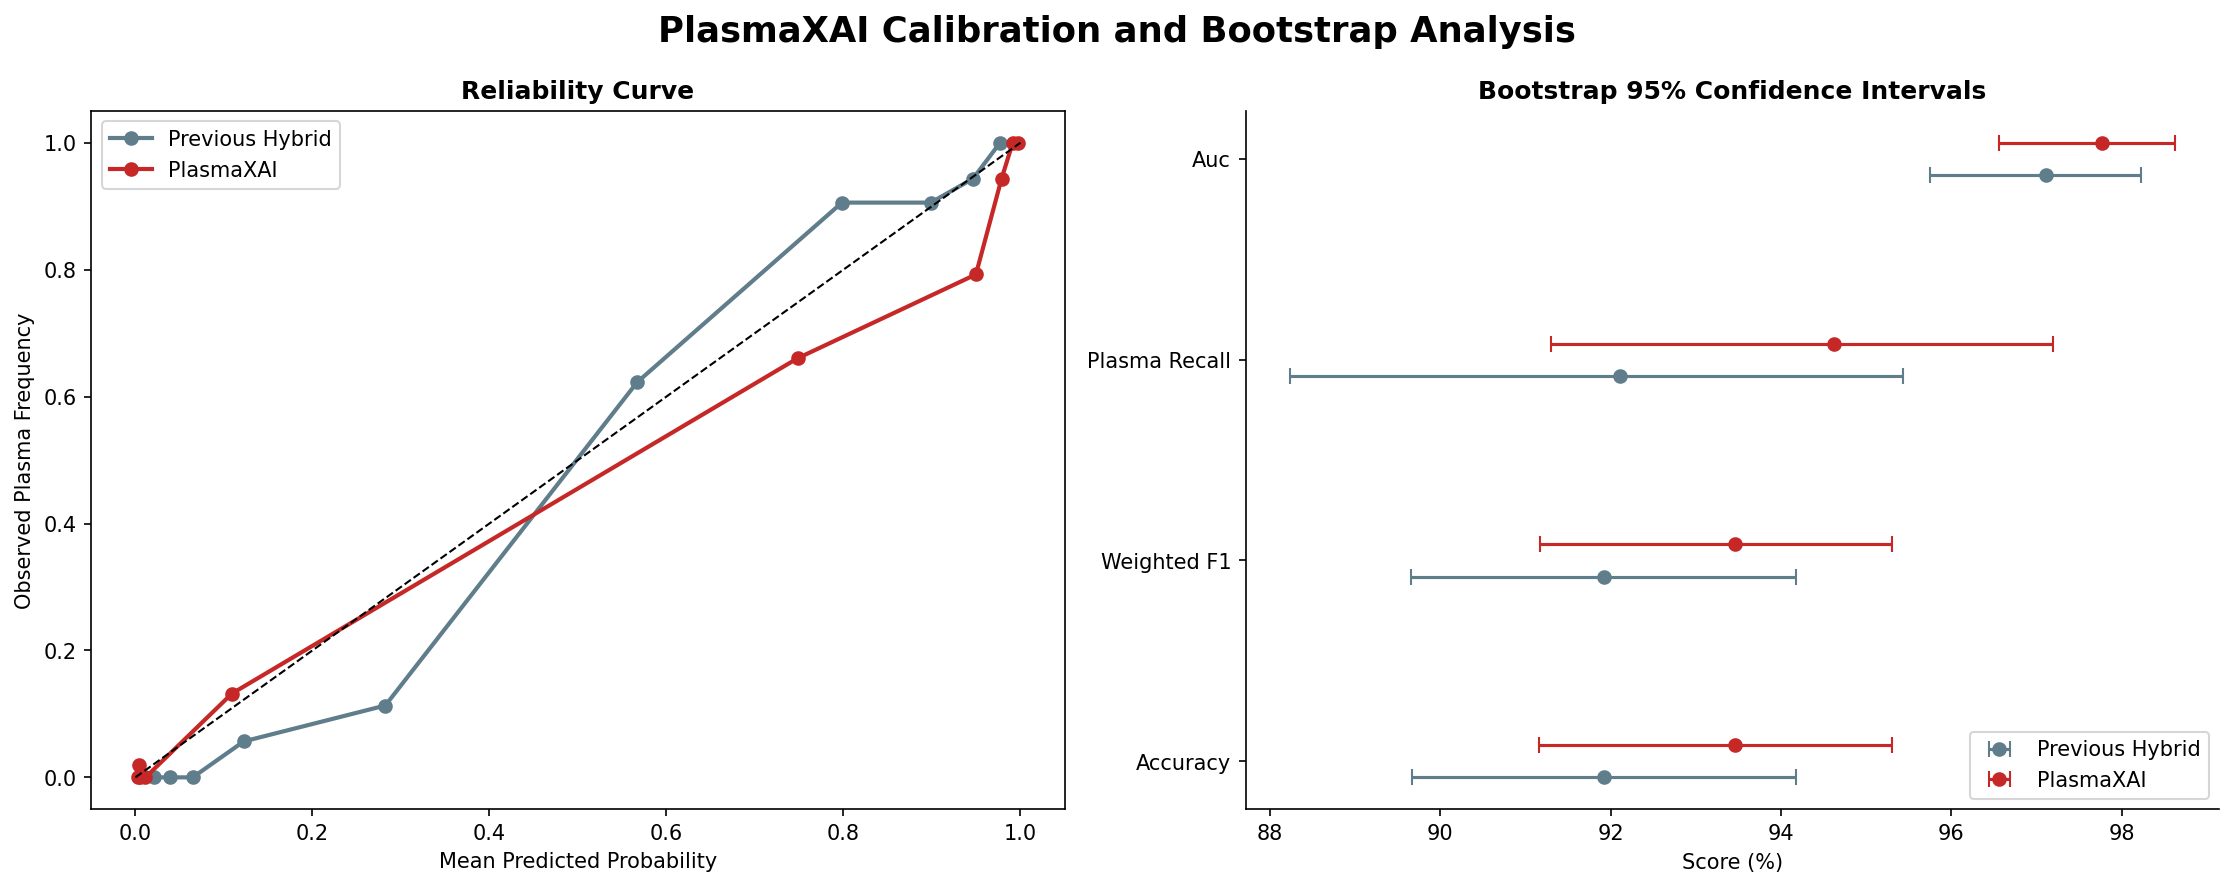
\includegraphics[width=0.90\textwidth,height=0.24\textheight,keepaspectratio]{plasmaxai_calibration_bootstrap.png}
\caption{Calibration curve and bootstrap stability analysis for PlasmaXAI.}
\label{fig:calibration}
\end{figure}
Figure~\ref{fig:calibration} shows that the selected operating point remains well behaved under repeated resampling.

\begin{figure}[t]
\centering
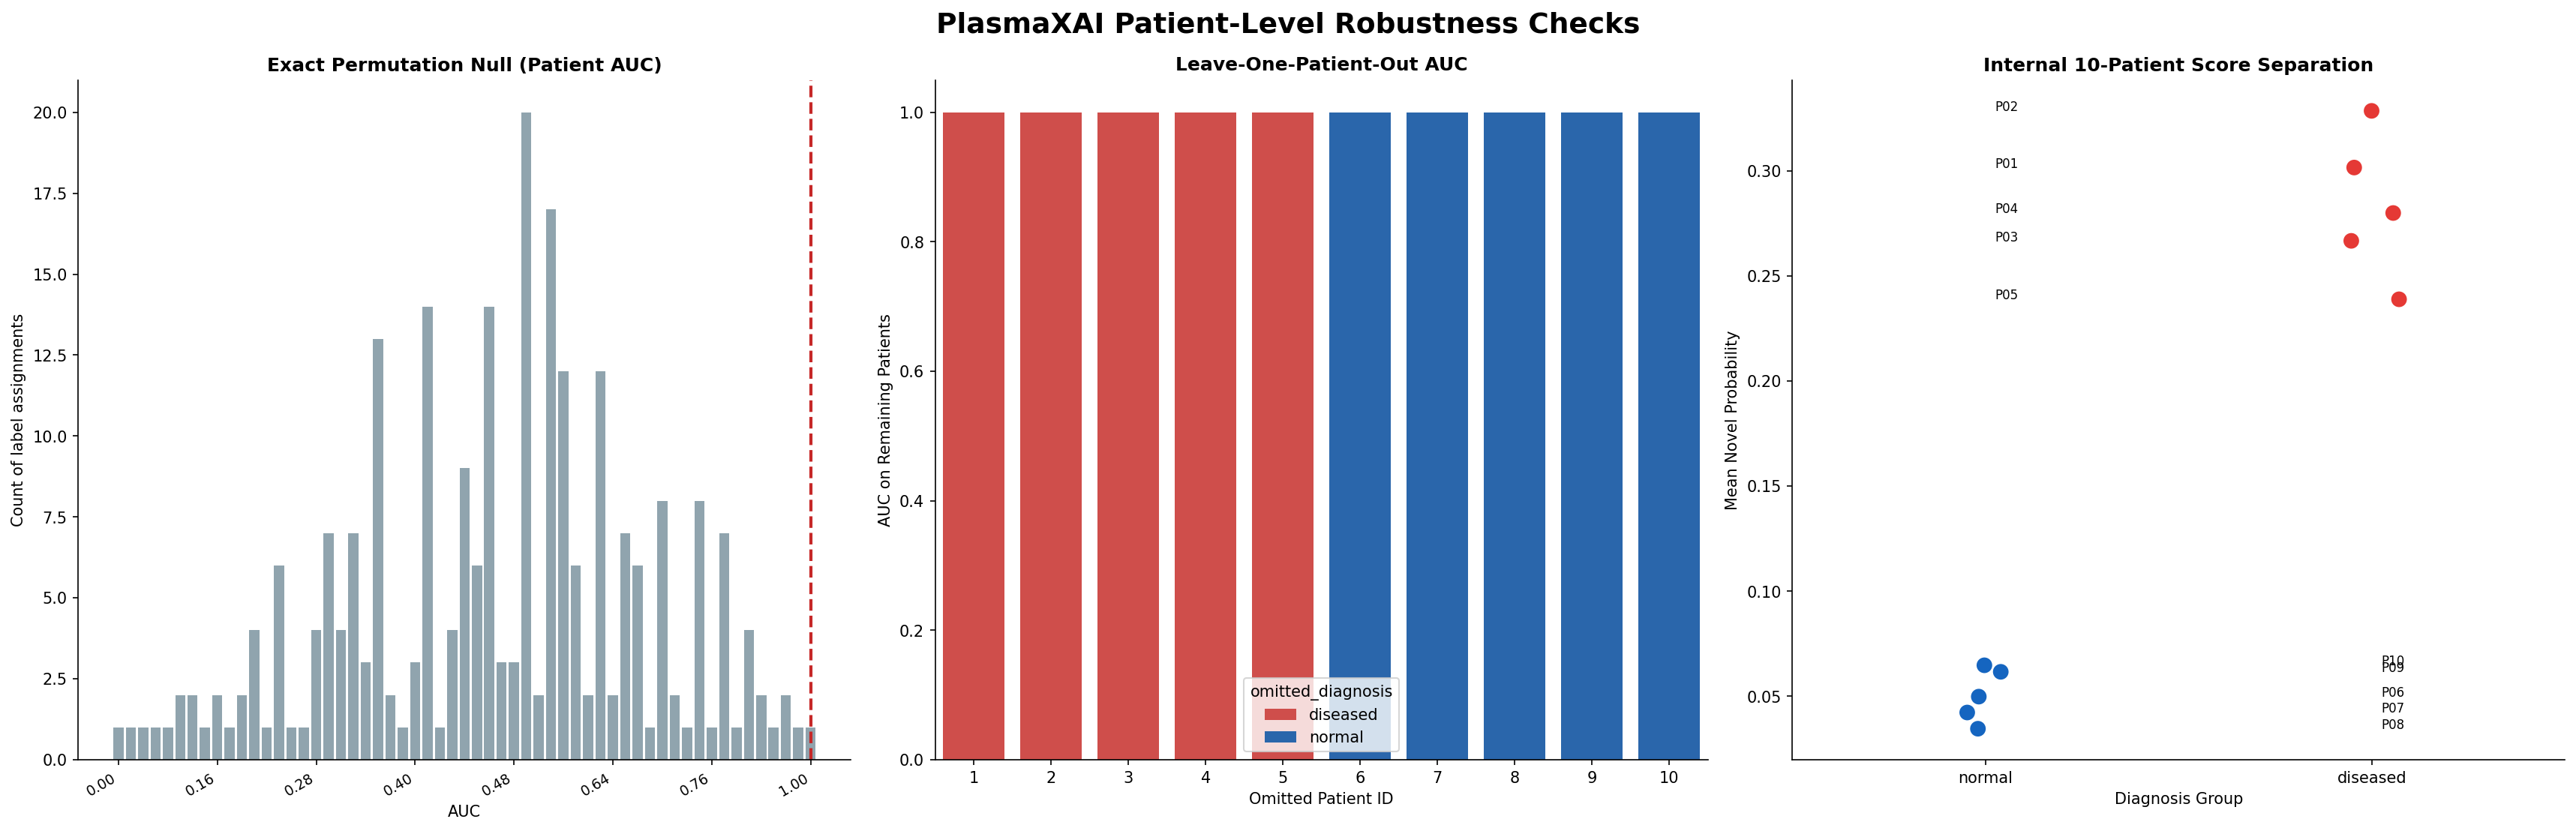
\includegraphics[width=0.90\textwidth,height=0.24\textheight,keepaspectratio]{plasmaxai_patient_robustness.png}
\caption{Patient-level robustness analysis using exact permutation testing and leave-one-patient-out evaluation.}
\label{fig:patientrobust}
\end{figure}
Figure~\ref{fig:patientrobust} highlights that the patient-level signal is strong internally, but should still be treated as exploratory.

\begin{figure}[t]
\centering
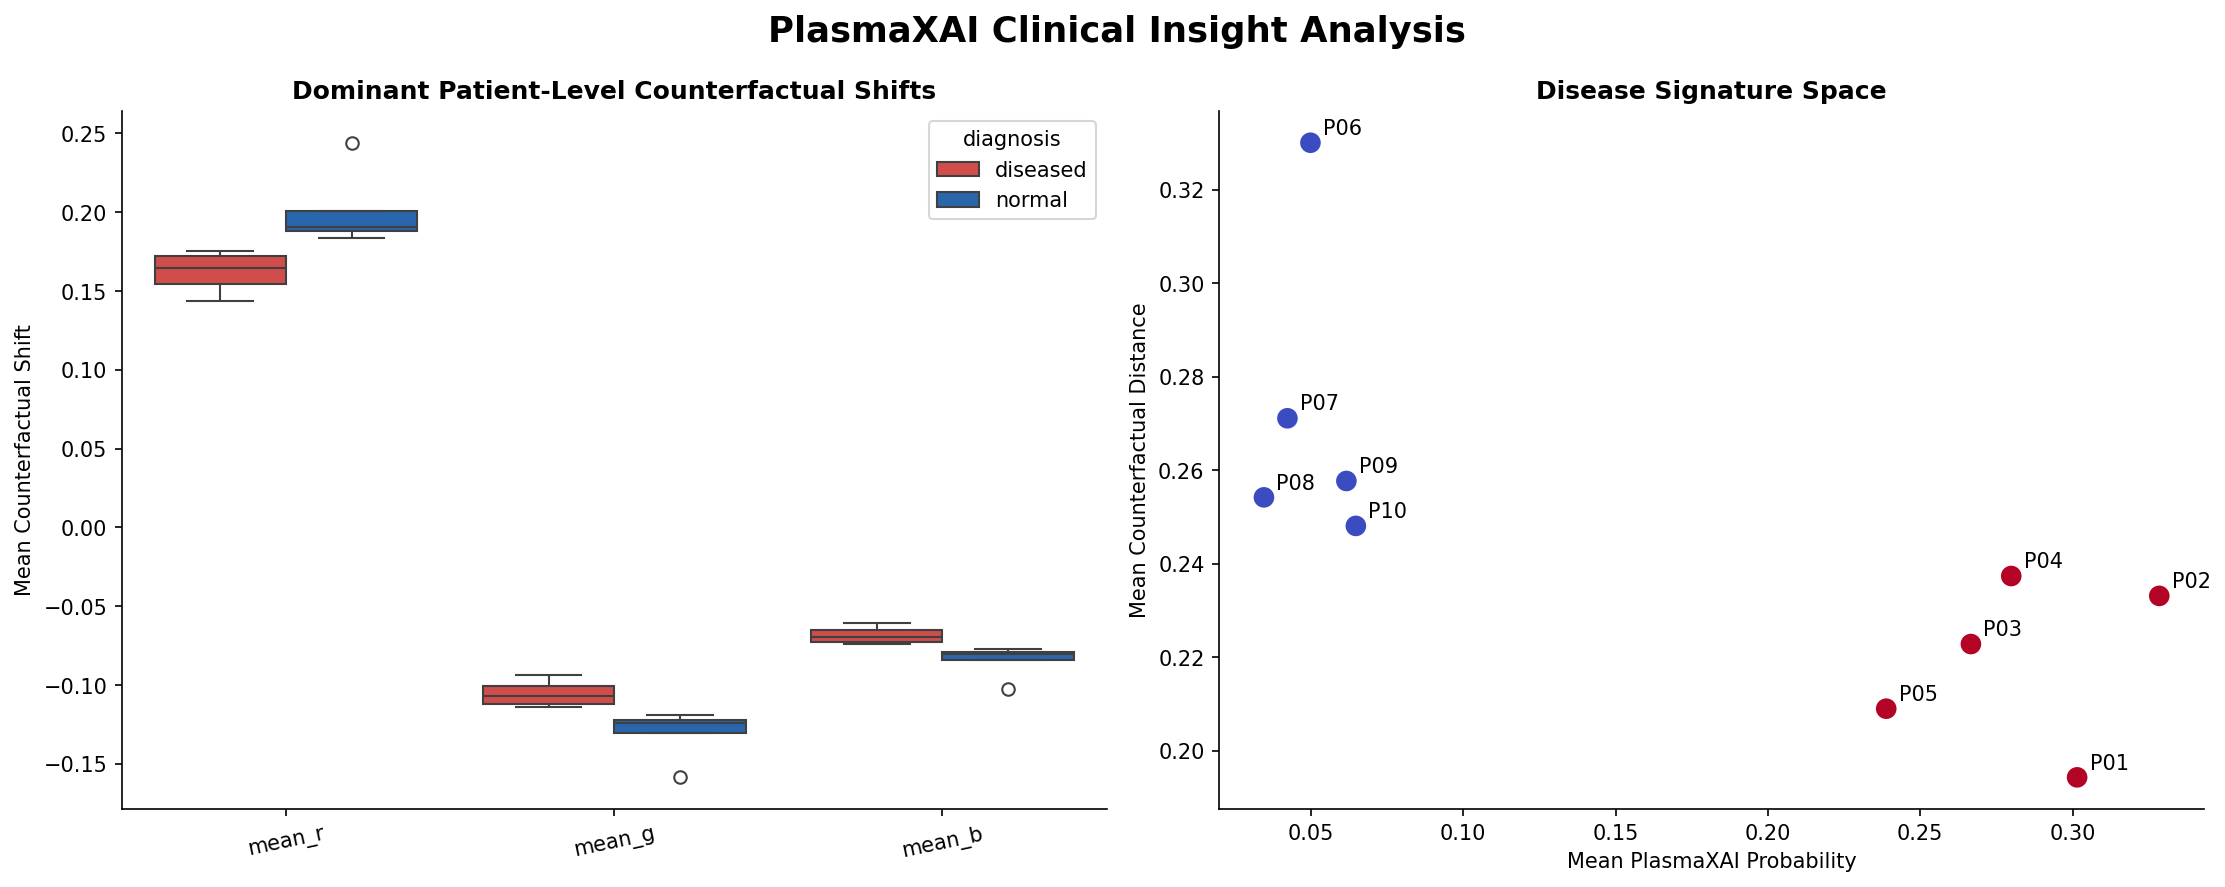
\includegraphics[width=0.90\textwidth,height=0.24\textheight,keepaspectratio]{plasmaxai_clinical_insight.png}
\caption{Clinical insight diagram summarizing the dominant disease-signature patterns discovered by PlasmaXAI.}
\label{fig:clinical}
\end{figure}
Figure~\ref{fig:clinical} summarizes the morphologic and chromatic patterns most associated with the malignant decision path.

\begin{figure}[t]
\centering
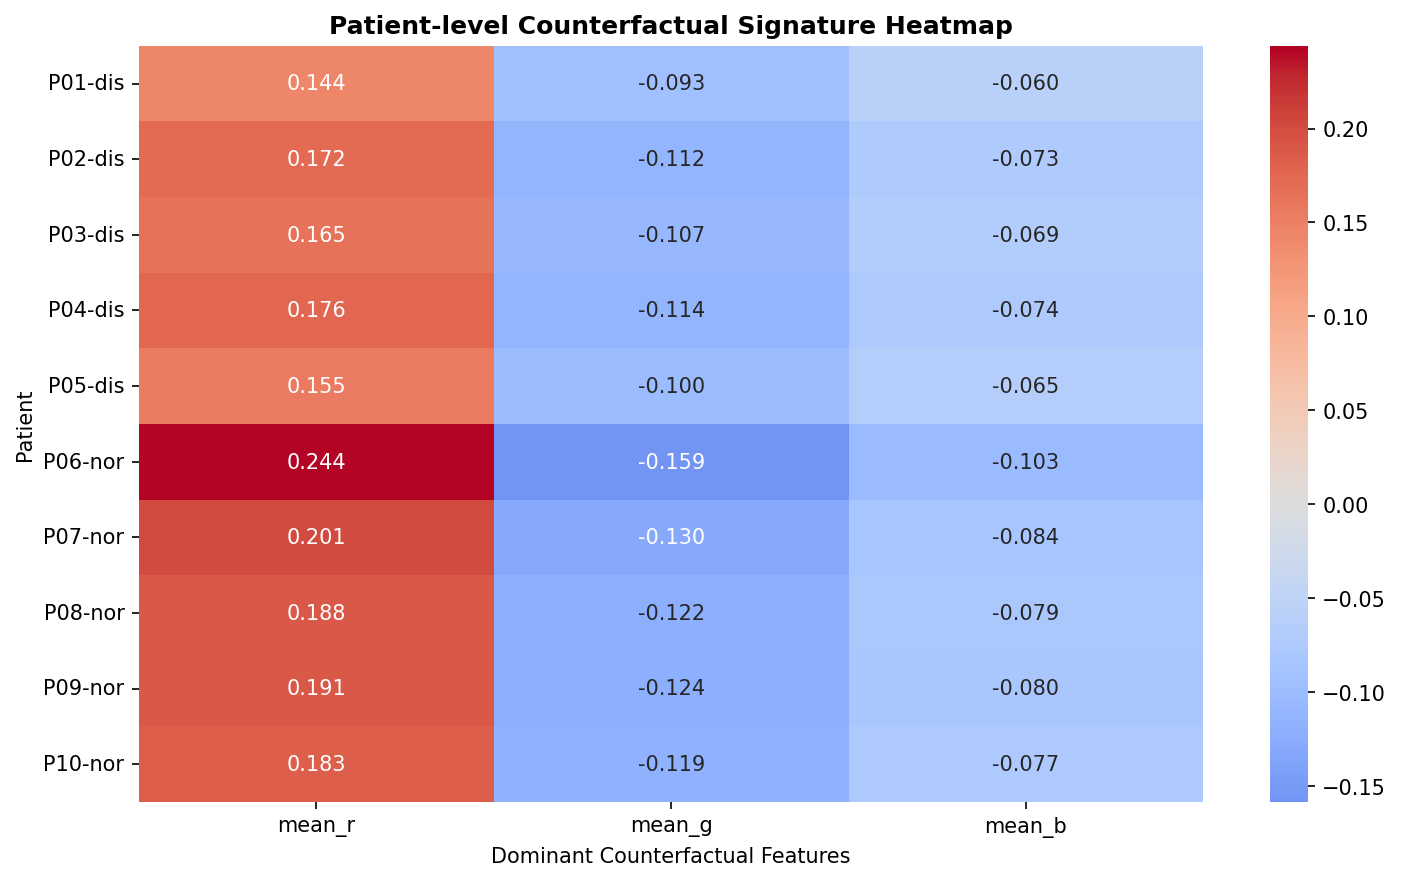
\includegraphics[width=0.90\textwidth,height=0.24\textheight,keepaspectratio]{plasmaxai_patient_heatmap.png}
\caption{Patient-level heatmap showing the consistency of disease-related morphology patterns across cases.}
\label{fig:heatmap}
\end{figure}
Figure~\ref{fig:heatmap} makes the patient-wise pattern consistency easier to inspect than a single scalar performance score.

Taken together, the results position PlasmaXAI as an explainable screening system rather than a narrowly optimized classifier. Its value lies in combining strong discrimination with traceable counterfactual reasoning and patient-wise consistency analysis.

\section{Conclusion}
This study presents PlasmaXAI as an explainable fusion framework for malignant plasma-cell recognition in multiple myeloma. By integrating deep image embeddings, interpretable morphology descriptors, and counterfactual signals inside a learned fusion pathway, the model achieves strong held-out performance while preserving transparency. PlasmaXAI outperforms key baselines, shows clear dependence on its counterfactual branch during ablation, and provides calibration, explanation, and patient-level analyses that support clinician-in-the-loop review. The main limitation is the lack of external multi-center validation. Future work should therefore emphasize stain-robust generalization, larger patient cohorts, and prospective hematopathology evaluation.

\begin{thebibliography}{99}
\bibitem{mmreview} Rajkumar, S.V.: Multiple myeloma: 2022 update on diagnosis, risk-stratification, and management. Am. J. Hematol. 97, 1086--1107 (2022)
\bibitem{litjens} Litjens, G., Kooi, T., Bejnordi, B.E., et al.: A survey on deep learning in medical image analysis. Med. Image Anal. 42, 60--88 (2017)
\bibitem{bera} Bera, K., Schalper, K.A., Rimm, D.L., Velcheti, V., Madabhushi, A.: Artificial intelligence in digital pathology---new tools for diagnosis and precision oncology. Nat. Rev. Clin. Oncol. 16, 703--715 (2019)
\bibitem{resnet} He, K., Zhang, X., Ren, S., Sun, J.: Deep residual learning for image recognition. In: Proceedings of the IEEE Conference on Computer Vision and Pattern Recognition, pp. 770--778 (2016)
\bibitem{densenet} Huang, G., Liu, Z., van der Maaten, L., Weinberger, K.Q.: Densely connected convolutional networks. In: Proceedings of the IEEE Conference on Computer Vision and Pattern Recognition, pp. 4700--4708 (2017)
\bibitem{wachter} Wachter, S., Mittelstadt, B., Russell, C.: Counterfactual explanations without opening the black box: Automated decisions and the GDPR. Harv. J. Law Technol. 31(2), 841--887 (2018)
\bibitem{diceml} Mothilal, R.K., Sharma, A., Tan, C.: Explaining machine learning classifiers through diverse counterfactual explanations. In: FAT* 2020, pp. 607--617 (2020)
\bibitem{calibration} Guo, C., Pleiss, G., Sun, Y., Weinberger, K.Q.: On calibration of modern neural networks. In: Proceedings of the 34th International Conference on Machine Learning, pp. 1321--1330 (2017)
\bibitem{unet} Ronneberger, O., Fischer, P., Brox, T.: U-Net: Convolutional networks for biomedical image segmentation. In: MICCAI 2015. LNCS, vol. 9351, pp. 234--241. Springer, Cham (2015)
\bibitem{attentionunet} Oktay, O., Schlemper, J., Folgoc, L.L., et al.: Attention U-Net: Learning where to look for the pancreas. arXiv preprint arXiv:1804.03999 (2018)
\bibitem{janowczyk} Janowczyk, A., Madabhushi, A.: Deep learning for digital pathology image analysis: A comprehensive tutorial with selected use cases. J. Pathol. Inform. 7, 29 (2016)
\bibitem{campanella} Campanella, G., Hanna, M.G., Geneslaw, L., et al.: Clinical-grade computational pathology using weakly supervised deep learning on whole slide images. Nat. Med. 25, 1301--1309 (2019)
\bibitem{lime} Ribeiro, M.T., Singh, S., Guestrin, C.: ``Why should I trust you?'': Explaining the predictions of any classifier. In: Proceedings of the 22nd ACM SIGKDD International Conference on Knowledge Discovery and Data Mining, pp. 1135--1144 (2016)
\bibitem{gradcam} Selvaraju, R.R., Cogswell, M., Das, A., et al.: Grad-CAM: Visual explanations from deep networks via gradient-based localization. In: Proceedings of the IEEE International Conference on Computer Vision, pp. 618--626 (2017)
\bibitem{shap} Lundberg, S.M., Lee, S.-I.: A unified approach to interpreting model predictions. In: Advances in Neural Information Processing Systems, pp. 4765--4774 (2017)
\end{thebibliography}

\end{document}
